% THIS DOCUMENT IS FOLLOWS THE VOLERE TEMPLATE BY Suzanne Robertson and James Robertson
% ONLY THE SECTION HEADINGS ARE PROVIDED
%
% Initial draft from https://github.com/Dieblich/volere
%
% Risks are removed because they are covered by the Hazard Analysis
\documentclass[12pt]{article}

\usepackage{booktabs}
\usepackage{tabularx}
\usepackage{hyperref}
\usepackage{float}
\usepackage{amsmath} 
\usepackage{multirow}
\usepackage{graphicx}
\hypersetup{
    bookmarks=true,         % show bookmarks bar?
      colorlinks=true,      % false: boxed links; true: colored links
    linkcolor=red,          % color of internal links (change box color with linkbordercolor)
    citecolor=green,        % color of links to bibliography
    filecolor=magenta,      % color of file links
    urlcolor=cyan           % color of external links
}

\newcommand{\lips}{\textit{Insert your content here.}}


\begin{document}

\title{Software Requirements Specification for \progname: Mission Control Terminal MC} 
\author{\authname}
\date{\today}
	
\maketitle

~\newpage

\pagenumbering{roman}

\tableofcontents

~\newpage

\section*{Revision History}
\begin{table}[hp]
\label{TblRevisionHistory}
\begin{tabularx}{\textwidth}{llX}
\toprule
\textbf{Date} & \textbf{Developer(s)} & \textbf{Change}\\
\midrule
October 6, 2023 & Q.H, R.V, D.A, D.C, U.R & Completed SRS documentation\\
October 9, 2023 & U.R & Added missing relevant facts and assumptions\\
October 20, 2023 & U.R & Added safety and security requirements from Hazard Analysis\\
November 3, 2023 & U.R & Added labels to FRs\\
\bottomrule
\end{tabularx}
\end{table}


~\\

~\newpage

\section{Introduction}
\subsection{Purpose of Document}
The purpose of this document is to explicitly define ground knowledge for the project, including definitions, context around the system, requirements, and more. This document is a collaborative effort across stakeholders, and aims to provide a clear and unambiguous understanding of the project’s purpose, functionality, and constraints.

\subsection{Scope of Requirements}
The scope of requirements is constraint to an application which operators can use to interact with various satellites, including, but not limited to, NEUDOSE, PRESET, and engineering test satellites. This project is not concerned with any other development that is currently undergoing at MIST.

\subsection{Characteristics of Intended Reader}
The intended reader is already familiar with the goals and objectives of the project, and might be reading this document for clarity around the project’s purpose, functionality, and constraints. Should the reader not be familiar with the project, please refer to the Problem Statement and Goals document found \href{https://github.com/RishiVaya/Lower_Earth_Orbiters/blob/main/docs/ProblemStatementAndGoals/ProblemStatement.pdf}{here} 

\section{Purpose of the Project}
\subsection{User Business}
The primary objective of our project is to provide satellite operators with a platform to automatically schedule and send commands to satellites as they pass overhead. In addition, the system will keep logs of all commands sent, responses, display polar plots with concurrent access available. 
\subsection{Goals of the Project}
See \href{https://github.com/RishiVaya/Lower_Earth_Orbiters/blob/main/docs/ProblemStatementAndGoals/ProblemStatement.pdf}{ Problem Statement and Goals document}, section 2.
\section{Stakeholders}
\subsection{Client}
\begin{itemize}
    \item Dr. Soohyun Byun
    \begin{itemize}
        \item Role: Supervisor and Principal Investigators at MIST.
        \item Interest: Dr. Byun, as the supervisor of this project, wants to ensure that the application facilitates efficient communication and success of the NEUDOSE and PRESET CubeSats.

        
    \end{itemize}

    \item Austin Liu
    \begin{itemize}
        \item Role: PRESET Systems Team Lead
        \item Interest: Austin is responsible for the overall system integration and performance of the PRESET CubeSat.

    \end{itemize}
\end{itemize}

\subsection{Customer}
\begin{itemize}
    \item McMaster Interdisciplinary Satellite Team (MIST)
    \begin{itemize}
        \item Role: Organization
        \item Interest: As the organization, their primary focus is on the success of the Mission Control Terminal application as it affects the entire satellite team’s operations. Their main concern is with the satellite operations and communication being reliable.

    \end{itemize}
    \item Any other Lower earth orbiting satellite commands or controls team
    \begin{itemize}
        \item Interest: Since the software will deal with satellite operation commands handling, any organization that sends lower earth satellites can be a customer of the software.

    \end{itemize}
    
\end{itemize}

\subsection{Other Stakeholders}
\begin{itemize}
    \item Muhammad Danyal
    \begin{itemize}
        \item Role: Software Specialist on Mission Operations and Control Team
        \item Interest: As a software specialist, Muhammad’s primary focus is in the functionality and usability of the Mission Control Terminal application.

    \end{itemize}
    \item Jay Patel
    \begin{itemize}
        \item Role: Command and Data Handling Team Leader
        \item Interest: Jay is interested in this project’s success as it directly relates to the handling of commands and data for the CubeSat.

    \end{itemize}
    \item Dr Eric Johnston and Dr Andrei Hanu
    \begin{itemize}
        \item Role: Principal Investigators of MIST
        \item Interest: As principal investigators of MIST, they will be one of the primary users of the data received from the satellite through MCT.
    \end{itemize}
\end{itemize}

\subsection{Societal Impact}
Our application is essential for society for several reasons. First, it directly supports the mission of the McMaster Interdisciplinary Satellite Team (MIST). This application can play a pivotal role for the success of MIST missions like NEUDOSE and PRESET by facilitating automatic scheduling and sending of commands to satellites as they orbit Earth. These missions are about understanding prolonged space radiation on human tissue and understanding the behaviour and impact it has on our atmosphere respectively. Our application can facilitate these missions thereby increasing the chance of these missions to being successful. The web-based interface makes the application accessible from various locations and devices, significantly improving accessibility and operational flexibility compared to traditional satellite control systems.

One significant advantage of this product over existing solutions is the user-friendly interface. It combines ease of use with the ability to schedule commands, predict satellite overpasses, and manage user authentication and authorization with modern protocols like OpenID Connect. This enhances operational efficiency and ensures secure, reliable satellite communication. Moreover, the application’s ability to log all commands and responses with different users is crucial for maintaining accurate records. 

It uses TLE data for accurate orbital predictions and incorporates UTF-8 character encoding for command exchanges, which enhances the system's robustness and fault tolerance. The web-based interface makes the application accessible from various locations and devices, significantly improving accessibility and flexibility compared to traditional satellite communication systems.


\subsection{Hands-On Users of the Project}
Operators have access to many functions that they previously didn't, and can act on these functions with the click of a button. They can perform the same actions as they did before, but with more efficiency and ease. 

\begin{itemize}
    \item Satellite Engineers
    \begin{itemize}
        \item Role: Engineers responsible for the operation of PRESET CubeSat, their next mission about understanding the behaviour of electrons and their impact on our atmosphere. 

        \item Interest: Satellite engineers may be involved in the testing and integration of the application with the satellite systems. This can help with understanding what aspects of the UI that maybe unclear or confusing.  

    \end{itemize}
    \item Command Operators
    \begin{itemize}
        \item Role: Users who utilize the application for mission control activities
        \item Interest: These are the end users of the Mission Control Terminal application. Their main focus is in the functionality, intuitiveness and responsiveness of the application.

    \end{itemize}
\end{itemize}

\subsection{Personas}
\begin{itemize}
    \item Application Administrators
    \begin{itemize}
        \item Responsible for user management where they can add, edit and define roles for operators
        \item Allowed to modify the permission list for each target and user.
    \end{itemize}

    \item Operators
    \begin{itemize}
        \item Users who are primarily scheduling commands to a target satellite. This includes creating, editing and deleting scheduled commands and sequences
    \end{itemize}
\end{itemize}
\subsection{Priorities Assigned to Users}
Ordering of priorities based on the different user roles:
\begin{itemize}
    \item Application Administrators: highest priority as they manage user and target access control.
    \item Operators: second and base role that a user can have. A user with this role is allowed to access the application and schedule commands to a target satellite.

\end{itemize}

\subsection{User Participation}
\begin{itemize}
    \item Operators: Operators are users who will be benefiting from this application and they will be actively interacting with the software application to schedule commands and gain data from the satellite. As a result, they will have a high involvement when ensuring the functionality of the application.
    \item Administrators: administrators will also have an active involvement in the usage of this software application. They will benefit by being able to easily manage user accounts in addition to scheduling commands to a target satellite. Therefore, the level of participation that application administrators have in this application is high.

\end{itemize}

\subsection{Maintenance Users and Service Technicians}
\begin{itemize}
    \item Muhammad Danyal and Mission operations and control team
    \begin{itemize}
        \item Role: Software Specialist on Mission Operations and Control Team
        \item Interest: As a software specialist, Muhammad’s primary focus is in the functionality and usability of the Mission Control Terminal application.

    \end{itemize}
\end{itemize}


\section{Mandated Constraints}
\subsection{Solution Constraints}
Solution Constraints are provided by MIST:
\begin{itemize}
  \item The MCT shall facilitate user creation and authentication through the OpenID Connect protocol.
  \item The MCT command port shall use the UTF-8 character encoding and exchange commands and data in plain text.
  \item The MCT shall use TLE (two-line element set) data periodically obtained from the internet to predict satellite overpasses and solar illumination cycles.
\end{itemize}

\section{Naming Conventions and Terminology}
\subsection{Glossary of All Terms, Including Acronyms, Used by Stakeholders
involved in the Project}
\begin{itemize}
    \item MCT - Mission Control Terminal
    \item MIST - McMaster Interdisciplinary Satellite Team
    \item NEUDOSE - Neutron Dosimetry \& Exploration (Satellite)
    \item PRESET - Pitch Resolving Spectroscopy for Electron Transport (Satellite)
    \item JSON - JavaScript Object Notation
    \item JWT - JSON Web Token
    \item Open standard to exchange security details over a network.
    \item GUI - Graphical User Interface
    \item CPU - Central Processing Unit
    \item RAM - Random Access Memory
    \item Disk space - The amount of storage that a computer hard disk/drive can store
    \item CI/CD - Continuous Integration/Continuous Development
    \item SSH - Secure Shell
    \item UTF-8 - Unicode Transform Format 8 bit
    \item Node.js - JavaScript runtime environment
    \item TypeScript - Extension of the JavaScript programming language which enforces strong typing
    \item Next.js - JavaScript framework for developing applications
    \item HIL Testing - Hardware in the Loop Testing
    \item Real-time simulation that allows for the testing of embedded systems
    \item Operator - Trained staff who are users of the application

\end{itemize}

\section{Relevant Facts And Assumptions}
\subsection{Relevant Facts}
\begin{itemize}
    \item UTF-8 does not produce conversion or loss of information when text is encoded in ASCII.
    \item OpenID Connect’s authentication protocol uses JSON Object Signing and Encryption (JOSE), including JSON Web Token (JWT) to encrypt information, which can be securely used for authorization and authentication flows.
    \item Github provides built-in support for Semantic Versioning.
    \item MongoDB offers auto-scaling capabilities, allowing for reactive vertical scaling.
    
\end{itemize}
\subsection{Business Rules}
\begin{itemize}
    \item Only users with the application administrator role can access and modify user data, such as permissions and roles
    \item Only authenticated and authorized users can send commands through the MCT.
    \item Logs of command sent to the satellite are stored in a database.
    The web application must be accessible through a web browser.
\end{itemize}

\subsection{Assumptions}
\begin{itemize}
    \item The application will be hosted on Linux-based servers.
    \item The application will not be hosted beyond a single server.
    \item The application does not store any science data collected by the satellite.
    \item Commands to operate the satellite will be provided to the application, where it does not need to design specific commands.
    \item The application will be compatible with commonly used web browsers, including Chrome, Firefox, and Edge.
\end{itemize}


\section{The Scope of the Product}
\subsection{Product Boundary}
\begin{figure}[H]
\centering
\caption{Scope and Out of Scope}
\begin{tabular}{|p{0.45\linewidth}|p{0.45\linewidth}|}
\hline
\textbf{In Scope} & \textbf{Out of Scope} \\
\hline
Command Scheduling: Operators need to be able to schedule commands for engineering and NEUDOSE satellites. They should be able to work concurrently with other users. & Satellite Hardware and Control Systems: The application will not directly interface with the satellite’s hardware; it will send commands to the ground station for transmission. \\
\hline
Orbital Prediction: Operators need to be able to calculate and predict satellite overpasses and satellite illumination cycles. & Ground Station Infrastructure: The application will not manage or control the ground station equipment. \\
\hline
User Authentication and Authorization: Users must be able to log in, with a special admin user which controls access to satellite usage. & Logging: Users must be able to retrieve a log of commands sent, and responses from the application. \\
\hline
\end{tabular}
\end{figure}
\subsection{Product Use Case Table}

\begin{table}[H]
\centering
\caption{User Use Cases}
\begin{tabular}{|p{0.45\linewidth}|p{0.45\linewidth}|}
\hline
\multicolumn{1}{|c|}{User} & \multicolumn{1}{c|}{Use Case} \\
\hline
\multirow{5}{*}{Operator} & - Schedule a set of commands to NEUDOSE and engineering test satellites via GUI \& Command Line \\
& - Modify \& Delete a set of commands to NEUDOSE and engineering test satellites \\
& - Access historical log data on satellite, operations, and responses \\
& - Login/Logout \\
& - View current orbital state for satellites of interest, and future overpasses \\
\hline
\multirow{2}{*}{Admin} & - Grant access to Operators on different access levels \\
& - Edit access permissions per operator \\
\hline
\end{tabular}
\end{table}
\subsection{System Boundaries}
.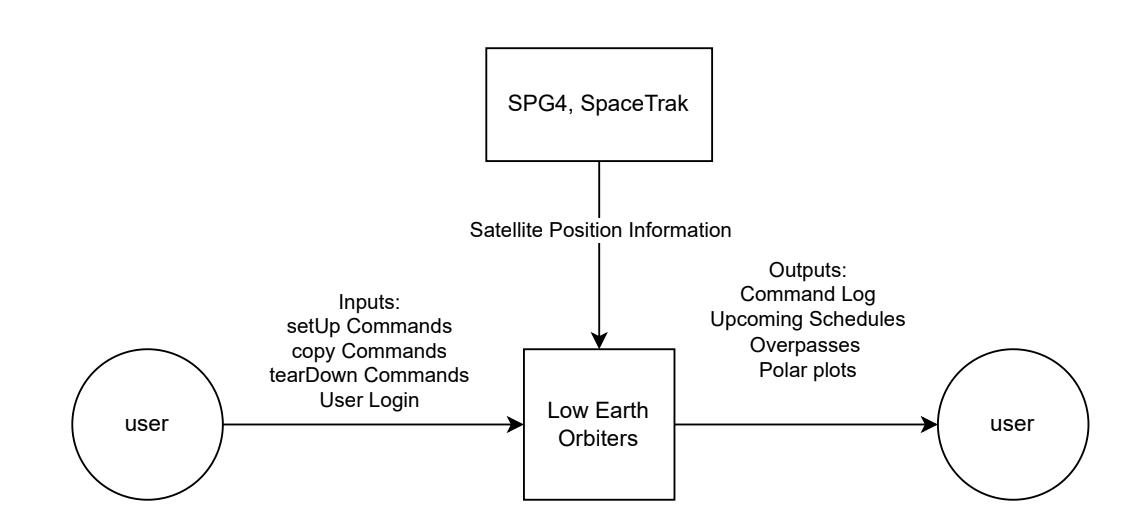
\includegraphics[width=15cm, height=10cm]{systemcontext.png}

\subsection{Formalized Math and the Application Flow }
  
\textbf{1. Commands Sent to the Satellite Must Be Encrypted}

\paragraph{Definitions:}
Let $C$ be the set of all commands that can be sent to satellites, $S$ be the set of all satellites, and $E$ be the set of all encrypted commands.\\

\textbf{Functions:}
\begin{itemize}
  \item Encryption: $f : C \rightarrow E$.
  \item Send: $g : E \times S \rightarrow \text{``Sent''}$.
\end{itemize}

\textbf{2. Users Sending Data to the Application}

\paragraph{Definitions:}
Let $U$ be the set of all users, $D$ be the set of all data items that users can send, and $A$ represent the application.\\


\textbf{Relation:}
\begin{itemize}
  \item Sending Relation: $R \subseteq (U \times D \times \{A\})$.
\end{itemize}

\textbf{3. Each Satellite Has Many Schedules}

\paragraph{Definitions:}
Let $S$ be the set of all satellites (as defined earlier) and $Sc$ be the set of all possible schedules.\\

\textbf{Relation:}
\begin{itemize}
  \item Scheduling Relation: $H \subseteq S \times Sc$.
\end{itemize}



\section{Functional Requirements}
\subsection{Functional Requirements}
\begin{enumerate}
    \item{FR-1\\}
    
    The MCT must run as a web application consisting of a graphical UI accessible through a web browser and TCP port to communicate commands. \\
    \textbf{Rationale:} We believe a web application is the most appropriate way to achieve communication between users and the satellite. We chose Linux because of its flexibility, reliability and overall security.
    
    \item{FR-2\\}
    
    The MCT must manage a list of users and its data, specifying the roles and all its associated actions. \\
    \textbf{Rationale:} This is to ensure that the system has a list of users to verify who’s allowed to enter and who isn’t. 

    \item{FR-3\\}
    

    The MCT will present a graphical interface allowing users to enter, select, and execute satellite commands while receiving text output from each command. \\
    \textbf{Rationale:} This is important because this is one of the most basic functions of our application, which includes three fundamental functions. The text output allows the user to understand the process as it’s happening so they are in the know. 

    \item{FR-4\\}
    
    The MCT will log all commands sent to and received from each target with timestamps. \\
    \textbf{Rationale:} This is helpful when the system runs into errors, because it’s easy to trace and determine what command caused it. 

    \item{FR-5\\}
    
    The MCT must present a graphical user interface to create, edit, and delete automated command sequences. \\
    \textbf{Rationale:} A graphical user interface enables intuitive interaction between the user and the system and improves the overall user experience. 

    \item{FR-6\\}
        
    The MCT must have an option to interrupt an executed command sequence during execution. \\
    \textbf{Rationale:} This is to allow the user to undo if a command was sent as a mistake or incorrect on their part. This will save plenty of time for the user rather than having to wait till the original command has been processed. 

    \item{FR-7\\}
    
    The MCT shall store a list of allowed commands and automated sequences for each target, specified using regular expressions. \\
    \textbf{Rationale:} This will ensure the system can verify a command when inputted by a user so that it matches to an allowed list. Otherwise, any command might influence a target which can cause damage.

    \item{FR-8\\}
        
    The MCT shall store a list of allowed commands and automated sequences for each user, specified using regular expressions. \\
    \textbf{Rationale:} This will ensure the system can verify the user so that it matches to an allowed list of users. Otherwise, any command by any user can negatively influence the satellite. 

    \item{FR-9\\}
    
    The application administrator shall be able to edit the permission list for each target and user. \\
    \textbf{Rationale:} An admin user who is responsible enough has been given permission to edit the list of targets and users. Without this functionality, if a user or command is attempting to cause damage it cannot be reprimanded. The admin user can remove or delete them to avoid said damage. 

    \item{FR-10\\}
    
    The MCT will be able to reject a user from executing a command unless that command matches the permission list criteria for the originating user. \\
    \textbf{Rationale:} This is vital because a command has to fit the permission list criteria in order for it to be allowed to run. Without this constraint, any command would be eligible to run which would be out of scope for this project. Specifically, it has to fit the criteria for that user group as different groups have different permissions for commands. 

    \item{FR-11\\}
    
    The MCT will be able to reject a user from executing a command unless that command matches the permission list criteria for the command target. \\
    \textbf{Rationale:} This is important because a command has to fit the permission list criteria for it to run. Specifically, it has to fit the criteria of commands for that command target, because each target has commands specifically associated to it. 

    \item{FR-12\\}
    
    The MCT must be able to schedule commands and automated command sequences for future execution. \\
    \textbf{Rationale:} This is important because a user may not have the time to wait or schedule a command for later. Through this, a user can save time to run commands without having to wait. 

    \item{FR-13\\}
        
    The MCT shall present a graphical user interface to create, edit, and delete scheduled commands and sequences. \\
    \textbf{Rationale:} A graphical user interface presents an intuitive interface for the user to interact with the satellite through create, edit and delete functions. A visual UI is most intuitive for every human to interpret and work with. 

    \item{FR-14\\}

    The MCT shall present a graphical user interface to select and edit the satellites of interest. \\
    \textbf{Rationale:} A graphical user interface presents an intuitive interface for the user to interact with the select and edit the satellites of interest. A graphical UI is most appropriate solution for this function.

    \item{FR-15\\}    

    The MCT shall display the current orbital state for satellites of interest, elevation, and solar illumination. \\
    \textbf{Rationale:} This is very important because it displays what the user is working with. For each satellite of interest, its elevation, orbital state and its illumination are vital pieces of information for the user to know. Presenting these on the screen is appropriate. 
    
    \item{FR-16\\}

    The MCT shall be able to schedule commands when a satellite enters a user-specified elevation threshold over the ground station coordinates. \\
    \textbf{Rationale:} This allows the user to manipulate any satellite within the threshold. This enables the user to play around with more satellites as their threshold is subject to preference. 

    \item{FR-17\\}
    
    The MCT shall be able to schedule commands when a satellite enters or exits in the covered area. \\
    \textbf{Rationale:} This is a core function of the application. The application can only manipulate and schedule commands for satellites within this area. Beyond this area would be too difficult for the application to manage. 

\end{enumerate}

\section{Look and Feel Requirements}
\subsection{Appearance Requirements}

\begin{itemize}
    \item \textbf{Look and feel:} The MCT look and feel should be consistent with the branding guidelines of MIST and the PRESET mission. This implies that the visual appearance and design aspects outlined by MIST and PRESET should be reflected in the user interface. The guidelines will be presented in section 5.3 of the Verification and Validation Plan document.
    \begin{itemize}
        \item \textbf{Rationale: }The client has outline this specification.
        \item \textbf{Phase in Plan}: This requirement will start phasing in at the time of designing the front-end of the application which starts after October 20, 2023.
    \end{itemize}
\end{itemize}


\subsection{Style Requirements}
\begin{itemize}
    \item N/A
\end{itemize}

\section{Usability and Humanity Requirements}
\subsection{Ease of Use Requirements}

\begin{itemize}
    \item \textbf{Ease of use:} The MCT web interface must be easy to use and accessible for all users, regardless of their level of technical expertise or disability.
    \begin{itemize}
        \item 
\textbf{Rationale: }It is essential to follow well-established usability and accessibility best practices, such as using clear and concise language, consistent design elements, and helpful feedback. 
\item \textbf{Phase in Plan}: This requirement will start phasing in at the time of designing the front-end of the application which starts after October 20, 2023.


    \end{itemize}
\end{itemize}


\subsection{Personalization and Internationalization Requirements}
\begin{itemize}
    \item N/A
\end{itemize}
\subsection{Learning Requirements}
\begin{itemize}
    \item 
\textbf{Ease of admin:} The MCT application should be easy to administer in order to reduce the workload on system administrators and make it easier to keep the system running smoothly.
\begin{itemize}
    \item \textbf{Rationale}: It is important to follow well-established administration best practices, such as using a centralized administration console, a simple and intuitive GUI, online support resources, and automation.
    \item \textbf{Phase in Plan}: This requirement will start phasing in at the time of designing the front-end and back-end of the application which starts after October 20, 2023.
\end{itemize}
\item 
\textbf{Documentation: }The MCT project should contain documentation for its web interface and key components. This documentation should be clear, concise, and easy to understand.
\begin{itemize}
    \item \textbf{Phase in Plan}: This requirement started phasing in at since the start of the project which was September 18th, 2023.
\end{itemize}
\item 
\textbf{Training: }An average user should take at most 10 minutes to understand how to use the MCT application.
\begin{itemize}
    \item \textbf{Rationale: }It is a good practice to make an application less complicated and easier to learn by using appropriate headings, layouts, themes etc.
    \item \textbf{Phase in Plan}: This requirement will start phasing in at when the application is ready for test deployment, which is February 5th, 2024.
\end{itemize}






\end{itemize}
\subsection{Understandability and Politeness Requirements}
\begin{itemize}
    \item N/A
\end{itemize}
\subsection{Accessibility Requirements}

\begin{itemize}
    \item \textbf{Compatibility: }The MCT web interface should be compatible with major browsers, operating systems and device types to ensure that all users, regardless of their preferred technology, can access and use the application effectively.
    \begin{itemize}
        \item \textbf{Rationale: }It is important to follow well-established web development best practices, such as using standard web technologies, avoiding browser-specific features, and testing the interface on a variety of devices and platforms.
        \item \textbf{Phase in Plan}: This requirement will start phasing in at the time of front-end development which starts after October 20th, 2023.
    \end{itemize}
\end{itemize}



\section{Performance Requirements}
\subsection{Speed and Latency Requirements}

\begin{itemize}
    \item \textbf{Responsiveness: }The MCT web interface should be responsive to user interactions. This is the measure of the time it takes for the interface to respond to user interactions.
    \begin{itemize}
        \item \textbf{Phase in Plan}: This requirement will start phasing in during the Verification and Validation phase, which is on November 3rd, 2023.
    \end{itemize}
    \item \textbf{Concurrent users:} The MCT should allow multiple users to access the service simultaneously to ensure that the latest information is displayed when a user hits refresh.
    \begin{itemize}
        \item \textbf{Phase in Plan}: This requirement will start phasing in at the deployment of the test application which is at February 5th, 2024.
    \end{itemize}
\end{itemize}


\subsection{Safety-Critical Requirements}

\begin{itemize}
    \item \textbf{Availability: }The MCT web service should be available outside of scheduled maintenance and not be affected by the availability of any targets.
    \begin{itemize}
        \item \textbf{Phase in Plan}: This requirement will start phasing in at when the application gets updates, which will be after its first test deployment on February 5th, 2024.
    \end{itemize}
\end{itemize}

\subsection{Precision or Accuracy Requirements}

\begin{itemize}
    \item \textbf{Time accuracy:} The MCT should ensure that the system date and time are accurate to the nanosecond as it is part of scientific research. The choice for the source will be presented in section 5.3 of the Verification and Validation Plan document.
    \begin{itemize}
        \item \textbf{Phase in Plan}: This requirement will start phasing in at the time of Verification and Validation Plan on November 3rd, 2023.
    \end{itemize}
    \item \textbf{Testing: }The MCT source code should have test suites to identify regressions and verify compliance with requirements. These test suites should support various features, including mocking, assertions, and parallel test execution.
    \begin{itemize}
        \item \textbf{Phase in Plan}: This requirement will start phasing in at the time of Verification and Validation Plan on November 3rd, 2023.
    \end{itemize}
\end{itemize}


\subsection{Robustness or Fault-Tolerance Requirements}

\begin{itemize}
    \item \textbf{Exceptions: }The MCT application should handle internal exceptions to ensure that the errors are catched when they occur during runtime.
    \begin{itemize}
        \item \textbf{Phase in Plan}: This requirement will start phasing in at the time of Verification and Validation Plan on November 3rd, 2023.
    \end{itemize}
\end{itemize}


\subsection{Capacity Requirements}

\begin{itemize}
    \item \textbf{Resource usage:} The MCT will minimize CPU, RAM, and disk space to be efficient.
    \begin{itemize}
        \item \textbf{Rationale: }It is a good practice to use efficient algorithms and data structures, requiring the system to use fewer resources.
        \item \textbf{Phase in Plan}: This requirement will start phasing in at the time of starting code which is after October 20th, 2023.
    \end{itemize}
\end{itemize}


\subsection{Scalability or Extensibility Requirements}
\begin{itemize}
    \item N/A
\end{itemize}
\subsection{Longevity Requirements}

\begin{itemize}
    \item \textbf{Service lifetime:} The MCT service should be operational until 2026, subject to extensions and improvements.
    \begin{itemize}
        \item \textbf{Rationale: }The client has outlined this specification.
        \item \textbf{Phase in Plan}: This requirement will start phasing in at 2026 when the application will no longer be maintained.
    \end{itemize}
\end{itemize}



\section{Operational and Environmental Requirements}
\subsection{Expected Physical Environment}
\begin{itemize}
    \item N/A
\end{itemize}
\subsection{Wider Environment Requirements}

\begin{itemize}
    \item \textbf{Staging environment:} A staging environment should be available to verify functionality before deploying to the production environment.
    \begin{itemize}
        \item \textbf{Rationale: }It is important to verify that the application is functioning before deploying to the production environment as it can catch any errors that might occur at production stage.
        \item \textbf{Phase in Plan}: This requirement will start phasing in at the first demonstration of the product, which is on February 5th, 2024.
    \end{itemize}
    \item \textbf{Development environment:} A local development environment for the MCT should be self-contained, meaning that the developer does not need to install any additional software or tools on their local machine to develop and test the application.
    \begin{itemize}
        \item \textbf{Phase in Plan}: This requirement will start phasing in at during the Verification and Validation Plan, on November 3rd, 2023.
    \end{itemize}
\end{itemize}


\subsection{Requirements for Interfacing with Adjacent Systems}
\begin{itemize}
    \item N/A
\end{itemize}
\subsection{Productization Requirements}
\begin{itemize}
    \item N/A
\end{itemize}
\subsection{Release Requirements}

\begin{itemize}
    \item \textbf{Commission date:} The MCT should be ready to use by September 2024.
    \begin{itemize}
        \item \textbf{Rationale: }The client has outlined this specification.
        \item \textbf{Phase in Plan}: This requirement will start phasing in at September 2024.
    \end{itemize}
\end{itemize}



\section{Maintainability and Support Requirements}
\subsection{Maintenance Requirements}

\begin{itemize}
    \item \textbf{Databases: }The MCT should use well-established database technologies to store application data and avoid text or plain files.
    \begin{itemize}
        \item \textbf{Rationale: }A well-established database is reliable and efficient. It is also essential to ensure data integrity, performance and scalability.
        \item \textbf{Phase in Plan}: This requirement started phasing in at the time of deciding the tools for the project, which was on September 25th, 2023.
    \end{itemize}
    \item \textbf{CI/CD process} The MCT should use a CI/CD process for software deployment and incorporate automated testing and static analysis. This is necessary to improve the speed and reliability of software deployments, to reduce the risk of human error, and to ensure the quality of the software.
    \begin{itemize}
        \item \textbf{Phase in Plan}: This requirement will start phasing in at during the Verification and Validation Plan, on November 3rd, 2023.
    \end{itemize}
    \item \textbf{System updates} The MCT should be able to update its libraries and dependencies to improve security, performance, or functionality.
    \begin{itemize}
        \item \textbf{Phase in Plan}: This requirement will start phasing in at during the Verification and Validation Plan, on November 3rd, 2023.
    \end{itemize}
    \item \textbf{Code quality:} The MCT source code should be well-organized, modular, and follow fundamental principles for software engineering. The standards will be defined in section 5.3 of the Verification and Validation Plan document.
    \begin{itemize}
        \item \textbf{Phase in Plan}: This requirement will start phasing in at the start of the code for the project, after October 20th, 2023.
    \end{itemize}
    \item \textbf{Code formatting:} The MCT source code should use a code formatting tool to ensure that the code is consistent and easy to read.
    \begin{itemize}
        \item \textbf{Rationale: }Since a project can have many contributors, it is important to be consistent with the style of code.
        \item \textbf{Phase in Plan}: This requirement will start phasing in at the start of the code for the project, after October 20th, 2023.
    \end{itemize}
    \item \textbf{Static analysis:} The MCT source code should use a linter or other static code analysis tools to catch errors and faults before runtime.
    \begin{itemize}
        \item \textbf{Phase in Plan}: This requirement will start phasing in at during the Verification and Validation Plan, on November 3rd, 2023.
    \end{itemize}
\end{itemize}


\subsection{Supportability Requirements}

\begin{itemize}
    \item \textbf{Containerization: }The MCT should be a containerized application in order to be portable, scalable, and efficient.
    \begin{itemize}
        \item \textbf{Rationale: }It is easier for a user to run tests on a containerized application as it does not require them to install any additional resources.
        \item \textbf{Phase in Plan}: This requirement will start phasing in at during the Verification and Validation Plan, on November 3rd, 2023.
    \end{itemize}
    \item \textbf{Backups: }The MCT should allow an administrator to back up its data to protect it from loss or corruption.
    \begin{itemize}
        \item \textbf{Phase in Plan}: This requirement will start phasing in at during the Verification and Validation Plan, on November 3rd, 2023.
    \end{itemize}
    \item \textbf{Application Logs:} The MCT application should store logs to facilitate debugging.
    \begin{itemize}
        \item \textbf{Rationale: }It is important to keep track of the logs in order to debug the application. This will also help in finding the methods/functions where an error occurs.
        \item \textbf{Phase in Plan}: This requirement will start phasing in after the Verification and Validation Plan, on November 3rd, 2023.
    \end{itemize}
\end{itemize}


\subsection{Adaptability Requirements}
\begin{itemize}
    \item N/A
\end{itemize}

\section{Security Requirements}
\subsection{Access Requirements}

\subsubsection*{AR-1:}
The application shall support multi-factor authentication such that a user must verify their identity through their registered email account. \\
\textbf{Rationale} Having multi-factor authentication provides an additional layer of security to the application, ensuring that unauthorized users are prohibited from accessing sensitive user and system data.
 \begin{itemize}
         \item \textbf{Phase in Plan}: This requirement will start phasing in after the system has completed every other core functionality, which will be a few days before February 5th, 2024.
         \item\textbf{This Access Requirement will no longer be implemented.}

    \end{itemize}


\subsubsection*{AR-2:}
The application shall not authenticate a user who has attempted to login with the same credentials ten times, consecutively. The application shall have a timeout period of five minutes before the user can authenticate themselves. \\
\textbf{Rationale} By having a timeout period for a set number of unsuccessful authentication attempts, it protects user accounts from unauthorized access and improves security.


\subsection{Integrity Requirements}
\subsubsection*{IR-1:}
The application shall periodically fetch TLE and calculate satellite overpasses to ensure the most recent data is being used to predict satellite overpasses. \\ 
\textbf{Rationale:} An issue with calculating satellite overpasses is the variation in TLE and other conditions. Periodically retrieving and recalculating this piece of information will ensure a more accurate prediction of overpasses.

\subsubsection*{IR-2:}
The application shall use a minimum elevation as a point of reference to evaluate whether a connection to the satellite can be made. \\
\textbf{Rationale:} In the case that a satellite is below the minimum elevation required to make a connection, the scheduled commands may not work and as a result, produce incomplete data. By having a minimum point of reference, the system can assess if a satellite is out of range.

\subsubsection*{IR-3:}
Operators shall be informed of errors that occur during the scheduling of commands, however, it is the operator’s responsibility to ensure the validity of the commands. \\
\textbf{Rationale:} Since the application allows operators to send and schedule commands to the satellite, it is possible that an incorrect command is sent.  In this case, it would be helpful to highlight the errors found in the operator’s input data.

\subsubsection*{IR-4:}
The system shall have a backup and recovery mechanism which is capable of restoring the database to its most recent correct state in the event of unexpected data failures. \\
\textbf{Rationale:} A situation may occur where the database enters into an unknown or corrupt state. The presence of a backup and recovery mechanism ensures that the information in the database is still accessible by rolling back to the most recent correct state.

\subsubsection*{IR-5}
In the event of a system, network, or satellite failure, all missing data fields shall be labelled with an appropriate error message as part of the data validation process. These error messages shall adhere to a standardized format. \\
\textbf{Rationale} There may be cases where a scheduled command produces responses with missing data attributes. By identifying the incomplete data using standardized error messages, it provides a consistent data state across all validation processes.

\subsubsection*{IR-6}
Cross-browser testing across a range of browsers shall be performed to ensure the application functions consistently. \\
\textbf{Rationale} Due to slight variations in browsers such as Safari, Chrome, and Firefox, it is important to assess the performance of the application across all user-intended environments.

\subsubsection*{IR-7}
The code base shall have HTML and CSS checks to ensure compatibility across different devices and browsers. \\
\textbf{Rationale} Incorporating the above checks can identify errors in the code base as well as possibly improve the application’s user interface.

\subsubsection*{IR-8}
All components which are required for scheduling operations shall be evaluated on their efficiency, where each component must complete within a minimum time frame. \\
\textbf{Rationale} By having a pipeline to test parts of the duration of a code, it can prevent situations where there may exist an inefficiency in scheduling operations.


\subsection{Privacy Requirements}

\begin{itemize}
    \item \textbf{Service security} Network ports exposed by the MCT should be secured using a reputed cryptographic protocol.
    \begin{itemize}
        \item \textbf{Phase in Plan}: This requirement will start phasing in at during the Verification and Validation Plan, on November 3rd, 2023. 
    \end{itemize}
\end{itemize}


\subsection{Audit Requirements}
\begin{itemize}
    \item N/A
\end{itemize}
\subsection{Immunity Requirements}
\begin{itemize}
    \item N/A
\end{itemize}

\section{Cultural Requirements}
\subsection{Cultural Requirements}
\begin{itemize}
    \item N/A
\end{itemize}

\section{Compliance Requirements}
\subsection{Legal Requirements}
\begin{itemize}
    \item For the scope of our project, all data and information that is used and being tracked is public information. Therefore, no legal or regulatory requirements exist for our application. 
\end{itemize}

\subsection{Standards Compliance Requirements}
\begin{itemize}
    \item Source code and releases should be version controlled adhering to the Semantic Versioning 2.0 standard
    \item Commands and data shall be encoded using UTF-8 character encoding standard
\end{itemize}

\section{Open Issues}
N/A

\section{Off-the-Shelf Solutions}
\subsection{Ready-Made Products}
\begin{itemize}
    \item Auth0 offers an authentication protocol that can be used to implement a user-based authentication flow for the application.
    \item SSH or TLS can be used as the cryptographic protocol to ensure security.
    \item ESLint is a linter that can be used to format and catch errors in the source code.
\end{itemize}

\subsection{Reusable Components}
\begin{itemize}
    \item Material UI is an open-source React component library which offers prebuilt user-interface components that can be used out-of-the-box.
\end{itemize}
\subsection{Products That Can Be Copied}
\begin{itemize}
    \item N/A
\end{itemize}

\section{New Problems}
\subsection{Effects on the Current Environment}
\begin{itemize}
    \item N/A
\end{itemize}

\subsection{Effects on the Installed Systems}
\begin{itemize}
    \item N/A
\end{itemize}

\subsection{Potential User Problems}
\begin{itemize}
    \item Accessibility to the command terminal requires authentication to be granted through the Auth0 Protocol. However, this is an industry-standard protocol for authentication and authorization, making it highly unlikely to encounter this problem.
\end{itemize}

\subsection{Limitations in the Anticipated Implementation Environment That May
Inhibit the New Product}
\begin{itemize}
    \item N/A
\end{itemize}

\subsection{Follow-Up Problems}
\begin{itemize}
    \item Currently the scope of this project is to be hosted on a single Linux server. However, extending this application to a generic MCT can cause data storage capacity issues when using the Free tier of MongoDB. This may require an upgrade in the tier of the database service.
\end{itemize}

\section{Tasks}
\subsection{Project Planning}
\begin{itemize}
    \item October 10, 2023: Revise requirements document
    \item October 20: Hazard Analysis
    \item November 3: Verification and Validation Plan
    \item November 13 - November 24: Form a Proof of Concept (POC)
    \item January 17: Design Document Revision
    \item March 8: Create a user documentation for the project
    \item March 18 - March 29: Final Demonstration 
\end{itemize}

\subsection{Planning of the Development Phases}

\textbf{Phase 1: Project Initiation and Planning}
\begin{itemize}
    \item Divide into two teams: Frontend and Backend

    \item October 20: Hazard Analysis
    \item Research into technology stack
        \begin{itemize}
            \item For frontend: Look into Next.js and TypeScript
            \item For Backend: Look into node.js and MongoDB Integration
            \item Authentication: Look into Auth0 protocol
            \item Set up testing, development, and production environments
        \end{itemize}
\end{itemize}

\textbf{Phase 2: Development}
\begin{itemize}
    \item Frontend
        \begin{itemize}
            \item Design mockups for the user interface and user experience (UI/UX)
            \item Build the frontend architecture
            \item Integrate APIs provided by the backend team
            \item Integrate client-side authentication and authorization
            \item Continuously test and debug frontend features
        \end{itemize}
    \item Backend
        \begin{itemize}
            \item Design database schema
            \item Implement security measures and role-based authorization
            \item Continuously test and debug backend endpoints
        \end{itemize}
\end{itemize}

\textbf{Phase 3: Integration Testing}
\begin{itemize}
    \item Perform testing to ensure the the functionality of the overall application is working as intended
    \item Identify and address issues
\end{itemize}

\textbf{Phase 4: Prototype Launch}
\begin{itemize}
    \item Gather feedback from Revision 0 Demonstration
    \item Address any issues or bugs identified
\end{itemize}

\textbf{Phase 5: Final Deployment and Launch}
\begin{itemize}
    \item Create user documentation and any required training materials
    \item Present the complete web-application 
\end{itemize}

\section{Migration to the New Product}
The purpose of this product is to develop MCT (Mission Control Terminal), a new web application with the following features and goals:
\begin{itemize}
    \item  Enable scheduling commands using built-in orbit prediction
    \item Unify control of the Engineering and Flight satellite models
    \item Facilitate operator training and hardware in the loop (HIL) testing
    \item Ensure storage and logs of commands sent to the satellite
    \item Manage operator accounts and access control
    \item Improve ease of use and accessibility of mission control software
\end{itemize}
\subsection{Requirements for Migration to the New Product}
Some changes will be required for the migration to the new product. Specific details about requirements will be updated during the development process.
\begin{itemize}
    \item Users will no longer need to access MCT from the machine at mission control. After the web application is live, users will have the freedom to access the MCT from any location.
    \item Strict role access will be implemented which will involve users to go through an authentication procedure to access MCT.
    \item The command communication process will migrate from the terminal to web based interface, making the application accessible to users of non-technical backgrounds.
 
\end{itemize}
\lips
\subsection{Data That Has to be Modified or Translated for the New System}
At this point, no data will require modification or translation

\section{Costs}
Provided below is a list of potential costs for the application. More details will be added as the project progresses
\begin{itemize}
    \item Server Cost - Since the application is a website, it will require a host to serve the application.
    \item Storage Cost - Having an extensive log of data collected and stored multiple times a day requires a large amount of storage space.

    \item Authentication Costs - Robust authentication might require use of external applications.
    \item Testing Cost - Testing the application will involve several steps which will include moving heavy machinery (Transmitters, receivers and the ground satellite).

\end{itemize}
\section{User Documentation and Training}
\subsection{User Documentation Requirements}
 The MCT project will contain documentation for its web interface and key components. This documentation will be clear, concise, and easy to understand.

\subsection{Training Requirements}
As a part of the final product, a training module will be added to the application. This training module will go through the components of the application and will allow a user to navigate through the system on a “test” satellite. Here, new users will have an opportunity to explore the system functionalities and get to test them, without affecting the 'real' satellites. 

\section{Waiting Room}
At this stage in the development cycle, there are no more requirements that will be added to the final product. This part of the document may be revised and updated as required during the development process.


\section{Ideas for Solution}
At this stage in the development cycle, there are no more requirements that will be added to the final product. This part of the document may be revised and updated as required during the development process.

\newpage{}
\section*{Appendix --- Reflection}

The information in this section will be used to evaluate the team members on the
graduate attribute of Lifelong Learning.  Please answer the following questions:

\begin{enumerate}
  \item What knowledge and skills will the team collectively need to acquire to
  successfully complete this capstone project?  Examples of possible knowledge
  to acquire include domain specific knowledge from the domain of your
  application, or software engineering knowledge, mechatronics knowledge or
  computer science knowledge.  Skills may be related to technology, or writing,
  or presentation, or team management, etc.  You should look to identify at
  least one item for each team member.
  \item For each of the knowledge areas and skills identified in the previous
  question, what are at least two approaches to acquiring the knowledge or
  mastering the skill?  Of the identified approaches, which will each team
  member pursue, and why did they make this choice?
\end{enumerate}

Quinn's Reflection
\begin{enumerate}
    \item Throughout this capstone project, will have to collectively learn various skills around project management, front-end/back-end development, devops, and more. Even with the collective years of experience of the team, building an entire system from scratch will prove to be a challenge. For me, I anticipate acquiring finer front-end development, UX and project management skills, due to my current interests in development, team management, and as they are skills needed for this project.

    \item Two approaches of learning front-end development and UX skills are online courses, and lots of development inside and outside the capstone project. These approaches are suitable for learning hard skills, and fill in the gap of knowledge that may exist. In addition, learning project management skills will be done through online courses, and speaking to professional project managers, to learn from. Project management as a skill is very personal to the individual, and being able to pick up tips and tricks from various professionals in the industry will ensure growth and eventually mastery of the skill.
\end{enumerate}

Diamond's Reflection
\begin{enumerate}
    \item To ensure the success of this project, the team will have to follow all of the Software Development Life Cycle (SDLC) principles. This includes processes from gathering requirements, designing, coding and implementation to deploying and maintenance. These process require skills like documentation, front-end / back-end development, CI/CD and good teamwork. My current interest is in the back-end development of our project and acquiring more skills relating to it such as Node.js and database integration. 

    \item I am currently taking a web-development course in which there are tutorials on developing a strong back-end for your web applications. It also shows integration with the database, which in our project is MongoDB. Another way is to make small personal projects to apply and refine the skills I currently have. I will pursue the first approach since back-end technology is very vast and our project is also time constrained which means creating small projects could result not being able to contribute to my full capacity to our capstone project.
\end{enumerate}


Dhruv's Reflection
\begin{enumerate}
    \item To complete this capstone project, our team will have to be well acquainted with various technologies, software languages and other skills such as testing and deployment. Although I have some experience working with front and back end applications, creating a project with this level of depth and requirements is new to me. I would like to work on my front end skills through online resources such as courses or checking out other's projects on GitHub. With this exposure, it would allow me to expand on my own creativity but also learn some tips and tricks. My interest would be more front end related because I find the creativity and aesthetic part of creating a great user interface very fun and challenging.  
    \item I would like to learn more about front end and back end through Youtube, online courses and by trying mini projects throughout the term. I believe that by practicing and actually building is the most effective way to learn. Although there are time constraints, enough mini courses and tutorials online can provide enough knowledge for me to build this capstone project well. 

\end{enumerate}


Rishi's Reflection
\begin{enumerate}
    \item The capstone project will require deep understanding of multiples technological and project management concepts. These concepts will be related to backend, frontend, databases and authentication on the software side, and Development cycles, continuous integration/continuous delivery (CI/CD) and documentation on the project management front. I would like to focus my development on the backend, databases and CI/CD. Although I have used these concepts during my internships and projects, I will need to acquire them in more detail for the successful completion of the capstone project.

    \item There are a lot of resources available to gain a better understanding of the technologies mentioned. These include online courses, youtube videos, numereous articles and help guides. By learning these concepts through the resources and continuously applying them in projects, I will be able to develop these skills in a capacity that will enable me to fullfill the project's requirements.
\end{enumerate}

Umang's Reflection
\begin{enumerate}
    \item 
        In order to make sure this project achieves all of its targeted goals, the team will have to become familiar when applying the software development principles, in conjunction with the technological and project management skills. The scope of this project involves real-life stakeholders which requires a level of organization and good communication to ensure certain goals are met. In addition, since this is also a software development process, developing a strong understanding of the technology stack will also help streamline the development process. As a group, we have to sharpen our concepts on the applications of the software development life cycle, as well as frontend, backend, and CI/CD technologies. I am aiming to build on my backend development skills, particularly Node.js and MongoDB's database service. While I do have some knowledge on these systems, I will have to be more fluent in these technologies in order to develop a successful product.

    \item There are several resources, whether it is in the form of books or videos, to learn more about the technologies and processes mentioned above. I will learn by reading through the documentation of the technologies, as well as online articles and possibly courses.
\end{enumerate}

Next steps:
\begin{itemize}
    \item Backend development courses and documentation: Rishi, Diamond and Umang will take the initiative to gain a deeper understanding of the backend development technologies by looking through available courses and documentation provided by Node.js and MongoDB.
    \item Frontend development courses and documentation: Quinn and Dhruv will take the initiative to gain a deeper understanding of the frontend development technologies by looking through available courses and documentation provided by TypeScript and Next.js.
    \item CI/CD courses: Dhruv and Diamond will take the initiative to gain a deeper understanding of the CI/CD through available courses and guides.
\end{itemize}

\end{document}